\documentclass[aspectratio=169,t,xcolor=table]{beamer}
\usepackage[utf8]{inputenc}

\usepackage{booktabs} 
\usepackage{subcaption}
\usepackage{epsfig}
\usepackage{siunitx}
\usepackage{physics}
\usepackage{setspace}
\usepackage{mathrsfs}
\usepackage{url}




\usetheme{UConn}

% ----------------------------------------------------------- Biblatex Citations
% \usepackage[
% backend=bibtex,
% style=ieee,
% ]{biblatex}
% \addbibresource{ECE5201_Citations.bib} %Imports bibliography file

% ------------------------------------------------------------- Bibtex Citations
% Optica Bibtex
\bibliographystyle{opticajnl}
\usepackage{jabbrv}
% \usepackage{footbib}

% \footbibliographystyle{opticajnl}
% \footbibliography{ECE5201_Citations}

% \usepackage{hanging}% http://ctan.org/pkg/hanging
% \setbeamertemplate{footnote}{%
%   \hangpara{2em}{1}%
%   \makebox[2em][l]{\insertfootnotemark}\footnotesize\insertfootnotetext\par%
% }

%-------------------------------------operators-------------
\newcommand{\dft}[2]{\frac{d^{#2}#1}{dt^{#2}}}
\DeclareMathOperator{\sinc}{sinc}
\DeclareMathOperator{\e}{e}
\DeclareMathOperator{\der}{d\hspace{-0.2em}}
\DeclareMathOperator{\proj}{proj}
\DeclareMathOperator{\sign}{sign}
\newcommand{\bX}[0]{\mathbf{X}}
\newcommand{\bv}[1]{\mathbf{#1}} 
\newcommand{\parallelsum}{\mathbin{\!/\mkern-5mu/\!}}
\newcommand{\vecc}[1]{\mathbf{#1}}

%-------------------------------------theorems--------------
\newtheorem{conj}{Conjetura}
\newtheorem{defi}{Definição}
\newtheorem{teo}{Teorema}
\newtheorem{lema}{Lema}
\newtheorem{prop}{Proposição}
\newtheorem{cor}{Corolário}
\newtheorem{ex}{Example}
\newtheorem{exer}{Exercício}

\setbeamertemplate{theorems}[numbered]
\setbeamertemplate{caption}[numbered]

%-------------------------------------------------------------%
%----------------------- Primary Definitions -----------------%

% This command set the default Color, is also possible to 
% choose a custom color
\setPrimaryColor{UConnBlue} 

% First one is logo in title slide (we recommend use a
% horizontal image), and second one is the logo used in the
% remaining slides (we recommend use a square image)
\setLogos{lib/logos/UConnHusky.png}{lib/logos/UConnHusky.png} 


% -------------------------------------- Title Slide Information
\begin{document}
\title{Electromagnetics \& Anisotropy}
% \subtitle{Kevin Lindstrom}
\institute{Department of Electrical and Computer Engineering\\
 University of Connecticut}
\subtitle{Half-Waveplates, Quarter-Waveplates, and Spatial Light Modulators}

\author{Kevin Lindstrom\\
\textrm{\href{mailto:kevin.lindstrom@uconn.edu}{kevin.lindstrom@uconn.edu}}}
\date{April 27, 2023}


%-----------------------The next statement creates the title page.
\frame[noframenumbering]{\titlepage}


%------------------------------------------------Slide 1
\setLayout{vertical} % This command define the layout. 'vertical' 
% can be replace with 'horizontal', 'blank, 'mainpoint', 'titlepage'

\begin{frame}
    \frametitle{Table of Contents}
    \tableofcontents
\end{frame}
%-------------------------------------------------------------------------------
% BEGIN PRESENTATION
% ------------------------------------------------------------------------------


%------------------------------------------------------------------ Introduction

% \begin{frame}
%     \frametitle{Objective}
%     % \vspace{-2.5em}
%     \cite{ELT_NLC}, \cite{PO}
% \end{frame}

\section{Theory}
\subsection{The Displacement Field}1
\begin{frame}
    \frametitle{The Displacement Field}
    The electric displacement field $\vecc{D}$ (with units 
    $\si{C\cdot m^{-2}}$) is defined as
    \begin{equation}\label{eq:D_deff}
        \vecc{D} = \epsilon_0 \vecc{E} + \vecc{P} 
        \color{red}
        = \epsilon \vecc{E}
        \color{black}
    \end{equation}
    where $\vecc{P}$ is the polarization of the material, and the \color{red} red
    \color{black} part of the equation is true given an isotropic dielectric
    \cite{griffithsEM}.\\
    \vspace{1em}
    The 
    \color{orange} perpendicular \color{black} and
    \color{blue} parallel \color{black} 
    boundary conditions (BC) for the displacement 
    field on an interface are
    \begin{equation}\label{eq:D_BC}
        \color{orange}
        (\vecc{D}_2 - \vecc{D}_1)\cdot \bv{\hat{n}}_{12} = \sigma_f
        \color{black}\quad\text{and}\quad\color{blue}
        (\vecc{D}_2 - \vecc{D}_1) \times \bv{\hat{n}}_{12} =
       (\vecc{P}_2 - \vecc{P}_1) \times \bv{\hat{n}}_{12}
       \color{black} 
    \end{equation}
    where $\sigma_f$ is the free (unbounded) surface charge density, and 
    $\bv{\hat{n}}_{12}$
    is the normal vector of the interface from medium 1 to medium 2.
\end{frame}

\subsection{Anisotropic Materials}
\begin{frame}
    \frametitle{The Displacement Field \& Anisotropy}
    \begin{alertblock}{What is Anisotropy?}
        Materials are \textit{Anisotropic} if their properties have 
        \textbf{directional
        dependence}. Specifically for us: a material's permittivity could take
        two different values depending on if the field is in the $\bv{\hat{x}}$ or
        $\bv{\hat{y}}$ directions \cite{Balanis-2012}.
    \end{alertblock}\\
    \vspace{1em}
    For anisotropic media, we use the relative permittivity tensor (rank 2), 
    which must be a Hermitian matrix \cite{CWA_S,Wav_anis}.
    \begin{equation}\label{eq:eps_ten}
        \bar{\epsilon}_r = \begin{bmatrix}
            \epsilon_{xx} & \epsilon_{xy} & \epsilon_{xz}\\
            \epsilon_{yx} & \epsilon_{yy} & \epsilon_{yz}\\
            \epsilon_{zx} & \epsilon_{zy} & \epsilon_{zz}\\
        \end{bmatrix}
        \quad\text{where}\quad
        \epsilon_{ij} = \epsilon_{ji}^*
    \end{equation}
    Equation \ref{eq:D_deff} becomes
    \begin{equation}\label{eq:D_anis}
        \vecc{D} =  \epsilon_0\bar{\epsilon}_r \vecc{E}
    \end{equation}
\end{frame}


\begin{frame}
    \frametitle{Uniaxial Media}
    Calcite, mica, and quartz are examples of \textit{uniaxial media}, where
    the permittivity tensor takes the form
    \begin{equation}\label{eq:PT_UA}
    \bar{\epsilon}_r = \begin{bmatrix}
        \epsilon^e & 0 & 0\\
        0 & \epsilon^o & 0\\
       0 & 0 & \epsilon^o\\
    \end{bmatrix}
\end{equation}
The $x$-axis is the \textit{extraordinary} axis, and $y$/$z$-axes 
are the \textit{ordinary} axes \cite{Wav_anis}.\\
\vspace{1em}
\begin{block}{Wave Propagation}
    We see that the permittivity in uniaxial media depends on the direction
    of the fields. Furthermore, we know the propagation constant depends on 
    the permittivity, and we will see that \textbf{waves propagate at different 
    speeds depending on their polarization}.
\end{block}
\end{frame}

\begin{frame}
    \frametitle{Half-Wave Plates}
    \begin{figure}[H]
        \centering
        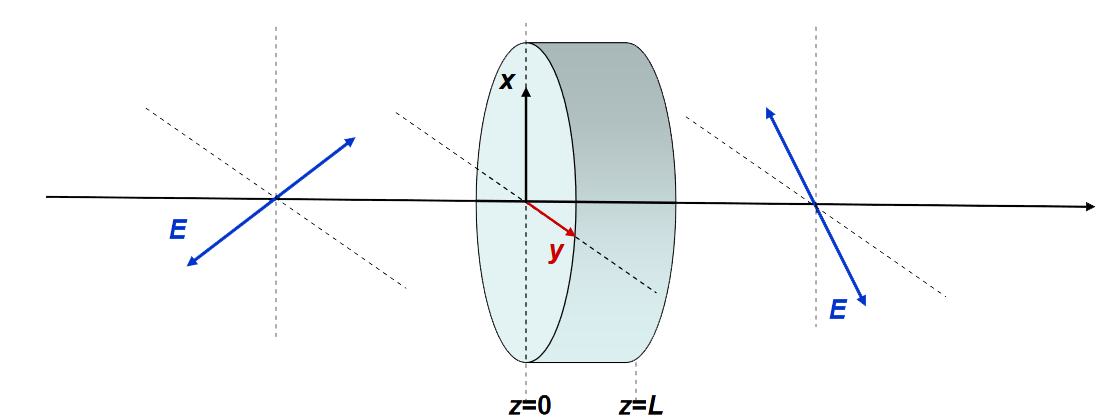
\includegraphics[width=\textwidth]{figs/HWP.PNG}
        \caption{
            A half-wave plate (HWP) in the $xy$-plane with length $L$ with an incident
            plane wave at $z=0$ \cite{Wav_anis}. HWPs rotate the polarization
            of an incident plane wave $\ang{90}$. We choose $z<0$ to be region 
            1, $0<z<L$ to be region 2, and $z>L$ to be region 3.
        }
    \end{figure}
\end{frame}


\begin{frame}
    \frametitle{The Wave Equation}
    Using Faraday's Law, Ampere's Law, and Equation \ref{eq:D_anis} we obtain
    the wave equation \cite{Wav_anis, Balanis-2012}
    \begin{equation}\label{eq:WaveEQ}
        \nabla \times \nabla \times \vecc{E}(\vecc{r}) = 
        -j\omega \mu_0 \nabla \times \vecc{H}(\vecc{r}) = 
    \omega^2\mu_0 \vecc{D}(\vecc{r})
    \end{equation}
    which becomes
    \begin{equation}\label{eq:WaveEQ_simp}
        \nabla^2 \vecc{E}(\vecc{r}) =  -\omega^2\mu_0 \vecc{D}(\vecc{r})
        = -\omega^2\mu_0\epsilon_0 \bar{\epsilon}_r \vecc{E}(\vecc{r})
    \end{equation}
    
    For normal incidence, a
    wave polarized in $\bv{\hat{x}}$ stays in $\bv{\hat{x}}$ in the dielectric
    \begin{equation}
        \vecc{E}_1(\vecc{r}) = \bv{\hat{x}}E_0 e^{-j\beta z}
        \quad\Rightarrow\quad
        \vecc{E}_2(\vecc{r}) = \bv{\hat{x}}T_{12}^{e}E_0 e^{-j\beta^e z}
        % \left(\frac{2\sqrt{1/\epsilon^e}}{\sqrt{1/\epsilon_0} +
        %  \sqrt{1/\epsilon^e}}\right)
    \end{equation}
    and $\bv{\hat{y}}$ stays in $\bv{\hat{y}}$
    \begin{equation}
    \vecc{E}_1(\vecc{r}) = \bv{\hat{y}}E_0 e^{-j\beta z}
        \quad\Rightarrow\quad
        \vecc{E}_2(\vecc{r}) = \bv{\hat{y}}T_{12}^{o}E_0 e^{-j\beta^o z}
    \end{equation}
\end{frame}

\begin{frame}
\frametitle{The Half-Wave Plate}
\begin{alertblock}{How do they work?}
    If for $\bv{\hat{x}}$ and $\bv{\hat{y}}$ incident polarization, the 
    polarization inside the dielectric does 
    not change, how does a HWP cause the polarization to change?
\end{alertblock}\\\vspace{1em}
Consider an incident wave LP in $\bv{\hat{x}}$ and $\bv{\hat{y}}$ \cite{Wav_anis}
\begin{equation}\label{eq:In_HWP}
    \vecc{E}_1(\vecc{r}) = 
    \left(\frac{\bv{\hat{x}} + \bv{\hat{y}}}{\sqrt{2}}\right)E_0 e^{-j\beta z}
    \Rightarrow
    \vecc{E}_2(\vecc{r}) = 
    \frac{E_0}{\sqrt{2}}\left(
        \bv{\hat{x}}T_{12}^{e} e^{-j\beta^e z} +
        \bv{\hat{y}}T_{12}^{o} e^{-j\beta^o z}
    \right)
\end{equation}
where 
\begin{equation}
\beta^e = \omega\sqrt{\mu_0\epsilon^e}
\quad\text{and}\quad
\beta^o = \omega\sqrt{\mu_0\epsilon^o}
\end{equation}
The field at $z=L$ becomes
\begin{equation}\label{eq:In_HWP_at_L}
    \left.\vecc{E}_2(\vecc{r}) \right|_{z = L}= 
    \frac{E_0}{\sqrt{2}}\left(
        \bv{\hat{x}}T^{e} e^{-j\beta^e L} +
        \bv{\hat{y}}T^{o} e^{-j\beta^o L}
    \right)
\end{equation}
\end{frame}

\begin{frame}
    \frametitle{The Half-Wave Plate Cont.} 
    For $\ang{90}$ polarization change we want to flip $\bv{\hat{x}}$ or 
    $\bv{\hat{y}}$, so we choose
    \begin{equation}\label{eq:L_HWP}
        L(\beta^o-\beta^e) = (2m+1)\pi
        \quad\mathrm{where}\quad
        m \in \mathbb{Z}
    \end{equation}
    such that equation \ref{eq:In_HWP_at_L} becomes \cite{Wav_anis}
    \begin{equation}\label{eq:Func_HWP}
        \left.\vecc{E}_2(\vecc{r}) \right|_{z = L}= 
        \frac{E_0}{\sqrt{2}}\left(
            \bv{\hat{x}}T^{e} e^{-j\beta^e L} +
            \bv{\hat{y}}T^{o} e^{-j\beta^o L}
        \right)
    \end{equation} 

    \end{frame}




\begin{frame}
    \frametitle{Citations}
    \vspace{-1.25em}
    \tiny
    % \printbibliography  % Biblatex
    \bibliography{ECE5201_Citations}  % Bibtex
    \vspace{1em}
        \textbf{Funding:}
        This research is currently unfunded.
      
        \textbf{Acknowledgments:}
        The author thanks T. Saule
        for his helpful contributions.
      
        \textbf{Disclosures:}
        The authors declare no conflicts of interest.
      
        \textbf{Data Availability:} Code for this project can be accessed on the
        author's github account. All of the current relevant data is shown in this
        report. Once a viable focus is achieved, the data will also be shown in the
        author's github as well.\\\vspace{1em}
        \textit{\href{https://github.com/kevinlindstrom/RMT_Simulation}
            {Simulation Repository} \&
            \href{https://github.com/kevinlindstrom/RMT_SLM}
            {Algorithm Code}}
\end{frame}


\setLayout{mainpoint}
%\setBGColor{UConnLightBlue}
\begin{frame}
    \frametitle{Questions?}
\end{frame}

\end{document}